\documentclass[11pt,letterpaper]{article}

\usepackage[utf8]{inputenc}
\usepackage[T1]{fontenc}
\usepackage{lmodern}
\usepackage[margin=1in]{geometry}
\usepackage{microtype}
\usepackage{amsmath, amssymb, amsthm, mathtools}
\usepackage{bm}
\usepackage{tikz, tikz-cd, pgfplots}
\usepackage{graphicx}
\usepackage[export]{adjustbox}
\usepackage{xcolor}
\PassOptionsToPackage{hyphens}{url}
\usepackage[colorlinks=true, allcolors=blue!50!black, breaklinks=true]{hyperref}
\usepackage[capitalize, noabbrev]{cleveref}
\usepackage{enumitem}
\usepackage[round, sort&compress]{natbib}
\usepackage{caption}
\usepackage{subcaption}
\usepackage{booktabs}
\usepackage{array}
\usepackage{titling}

\pgfplotsset{compat=1.18}
\usetikzlibrary{positioning, arrows.meta, cd, fit, backgrounds, calc, matrix,
  shapes.geometric, decorations.pathreplacing, shapes.misc, patterns}

\emergencystretch=3em
\hbadness=2000
\tolerance=1000

% --- Okabe--Ito accessible palette ---
\definecolor{okBlack}{HTML}{000000}
\definecolor{okOrange}{HTML}{E69F00}
\definecolor{okSky}{HTML}{56B4E9}
\definecolor{okGreen}{HTML}{009E73}
\definecolor{okYellow}{HTML}{F0E442}
\definecolor{okBlue}{HTML}{0072B2}
\definecolor{okVerm}{HTML}{D55E00}
\definecolor{okPurple}{HTML}{CC79A7}

\tikzset{
  every node/.style={font=\sffamily\small},
  arr/.style={-Stealth, semithick},
  arrd/.style={-Stealth, semithick, dashed},
  obj/.style={draw, rounded corners=2pt, inner sep=5pt, font=\sffamily\small, align=center},
  box/.style={draw, rounded corners=2pt, inner sep=4pt, font=\sffamily\footnotesize, align=center},
  boxBlue/.style={box, fill=okBlue!12, draw=okBlue},
  boxGreen/.style={box, fill=okGreen!14, draw=okGreen!80!black},
  boxOrange/.style={box, fill=okOrange!18, draw=okOrange!80!black},
  boxPurple/.style={box, fill=okPurple!16, draw=okPurple!80!black},
  seed/.style={draw, circle, minimum size=8mm, fill=okYellow!60, line width=0.9pt,
               font=\sffamily\scriptsize, align=center},
  pt/.style={draw, circle, minimum size=4.4mm, inner sep=0pt, font=\sffamily\scriptsize},
}

\theoremstyle{plain}
\newtheorem{theorem}{Theorem}[section]
\newtheorem{lemma}[theorem]{Lemma}
\newtheorem{proposition}[theorem]{Proposition}
\newtheorem{corollary}[theorem]{Corollary}
\theoremstyle{definition}
\newtheorem{definition}[theorem]{Definition}
\newtheorem{example}[theorem]{Example}
\theoremstyle{remark}
\newtheorem{remark}[theorem]{Remark}

% --- cohesion + type-theoretic notation (font-safe) ---
\newcommand{\shapeM}{\mathop{\mathsf{S}}\nolimits}      % shape modality (Shulman's esh)
\newcommand{\flatM}{\mathop{\flat}\nolimits}            % flat modality
\newcommand{\sharpM}{\mathop{\sharp}\nolimits}          % sharp modality
\newcommand{\Bd}{\partial}                              % the two-point boundary
\newcommand{\ua}{\mathsf{ua}}                           % univalence (cubical)
\newcommand{\transport}{\mathsf{transp}}
\newcommand{\isContr}{\mathsf{isContr}}
\newcommand{\PiZero}{\Pi_0}                             % connected components
\newcommand{\Disc}{\mathrm{Disc}}
\newcommand{\Gam}{\Gamma}
\newcommand{\coDisc}{\mathrm{coDisc}}
\newcommand{\NN}{\mathbb{N}}
\newcommand{\ZZ}{\mathbb{Z}}
\newcommand{\QQ}{\mathbb{Q}}
\newcommand{\RR}{\mathbb{R}}
\newcommand{\Zphi}{\ZZ[\varphi]}
\newcommand{\bbtwo}{\mathbb{Z}/2}
\newcommand{\fib}{\mathrm{F}}                           % Fibonacci
\newcommand{\unmk}{\mathsf{u}}                          % unmarked
\newcommand{\mkd}{\mathsf{m}}                           % marked
\newcommand{\cross}{\sigma}                             % the Laws-of-Form crossing
\newcommand{\modulus}{\mu}
\newcommand{\Llog}{h}                                   % logical entropy
\DeclareMathOperator{\Hom}{Hom}
\DeclareMathOperator{\Iso}{Iso}
\DeclareMathOperator{\colim}{colim}
\DeclareMathOperator{\Carrier}{Carrier}

\newif\ifIAOMPublication
\ifdefined\IAOMPUBLICATION
  \IAOMPublicationtrue
\else
  \IAOMPublicationfalse
\fi

\begin{document}

% =========================================================================
% TITLE PAGE
% =========================================================================
\begin{titlingpage}
\centering
\vspace*{0.3em}

{\huge\bfseries Every Limit a Corridor\par}

\vspace{0.45em}
{\Large A Constructive Engine for Effective Mathematics\par}

\vspace{0.9em}

\includegraphics[width=0.16\textwidth]{figures/IAOM_logo.png}

\vspace{0.45em}
{\normalsize\scshape \href{https://www.apoth3osis.io/IAOM}{Institute for Applied Ontological Mathematics}\par}

\vspace{0.25em}
{\footnotesize June 2026\par}

\vspace{0.8em}
\begin{minipage}{0.90\textwidth}
\footnotesize
\textbf{Abstract.}\quad
Classical analysis hands you a \emph{point}: a limit exists, but the theorem is
silent on how many steps it takes to reach it, or what that reaching costs.
Effective mathematics replaces the point with a \emph{corridor}---a two-sided
bracket carried as data, narrowing at an intrinsic rate. The width is not
metadata about the object; it \emph{is} the object. In a physicist's terms, the
corridor is a wavepacket whose error bars are intrinsic and computable rather
than imposed by hand. We take a concrete proposal---synthesize a point-free
``$\QQ$-free ladder,'' a bi-Lipschitz spectral corridor, and the computability
certificates of Eagle and McNicholl---and realize it as one instance of the
Institute's build-from-Nothing engine, in \emph{cohesive homotopy type theory},
then lower it to a bare-metal artifact. Five constructions carry the
result, each a genuine mathematical object. \textbf{(i)} A faithful real-cohesion
in which the two walls are genuinely different functors: the continuity wall
($\shapeM$) collapses the corridor's endpoints to a single connected point, while
the cost wall ($\flatM$) keeps them apart---topology and distinguishability,
separated, with no metric required. \textbf{(ii)} A univalence that
\emph{computes}: the Laws-of-Form re-entry is realized as an involution whose
transport flips the boundary state, exactly as a reflection acts on a two-level
system, and the identification is a path that runs rather than an axiom that
sticks. \textbf{(iii)} A golden-ratio modulus that makes ``the ladder is the
rate'' a theorem---the Fibonacci ladder reaches any precision, and a
\emph{constant} rate is provably refuted, so convergence cannot be faked; this is
Veselov's lower certificate, the bound that forbids collapse to the syntactic
horizon. \textbf{(iv)} An approximately-finite colimit over $\Zphi$ whose stages
are those same golden brackets. \textbf{(v)} An $H^1$ logical-entropy screen: the
re-entry loop carries a cohomology class that is locally a coboundary but globally
nontrivial, of order two, with strictly positive logical entropy---a topological
charge no continuous deformation removes, measured in the same logical-entropy
currency the engine uses to weigh a number's provenance. One identity binds them:
the colimit's approximants \emph{are} the modulus's brackets. The whole programme
then leaves the page: every construction lowers to a bare-metal interaction-net
program, and the result is admitted as executable-form closure through a lane
gated by a \emph{negative control}---a degenerate witness the kernel provably
rejects---so the certificate records that the object reaches executable bare-metal
form past a discriminating gate, not merely that it type-checks (and its key
computation, the univalence transport, reduces in the kernel besides). We argue
throughout that homotopy type theory is not incidental but
essential: univalence supplies the computing identification, cohesion supplies the
two walls without a metric, and higher inductive types supply the loop, the
quotient, and the colimit as first-class objects rather than encodings. Beyond the
representative models, the formalization carries the analytic real line $\RR$ on
which the two walls separate, and the golden value as a located, \emph{irrational}
real $\varphi:\RR$ with its conjugate and forced modulus
(\cref{sec:formalization}); the $C^\ast$-norm is established on the algebra's
commutative core, leaving the non-commutative operator-norm completion as the one
remaining part.
\end{minipage}

\end{titlingpage}

% =========================================================================
\section{The point and the corridor}\label{sec:intro}

\paragraph{The question.}
What does it cost to reach a limit? Ordinary analysis does not ask. It proves
that a Cauchy sequence converges, that a spectrum is nonempty, that an operator
has a square root---and then falls silent. The object \emph{exists}; the manner
of its existence is treated as none of mathematics' business. But a physicist
computing a scattering amplitude, an engineer certifying a control loop, and a
proof assistant checking a bound all need the manner: how many digits, after how
many steps, at what guaranteed rate. A limit that merely exists is a promissory
note. A limit you can \emph{use} is a promissory note with a payment schedule
attached.

This paper is about attaching the schedule---and discovering that, once attached,
it stops being an annotation and becomes the object itself.

\paragraph{The claim.}
Replace the point by a \emph{corridor}: a pair of walls bracketing the target
from below and above, together with a rule---a \emph{modulus}---that says how fast
the walls close. Three things then become true at once, and we prove all three
inside a single proof kernel.

First, the two walls are not the same kind of thing. One wall is
\emph{continuity}: it is cheap, it is topological, and in the cohesive setting it
is the image of the \emph{shape} modality, which sees only connectedness. The
other wall is \emph{cost}: it is where the constructive work lives, it is the
image of the \emph{flat} modality, and it is what keeps two genuinely distinct
states from being silently identified. We exhibit a model in which these two
modalities are provably different functors---the shape of the corridor's interval
is a single connected point, while its flat keeps the two endpoints apart---so the
separation of topology from distinguishability is a theorem, not a slogan, and it
needs no metric to state.

Second, the modulus is forced. We build the rate from the golden ladder---a
point-free, $\QQ$-free, zero-free inductive scaffold---and prove that it reaches
any demanded precision while a \emph{constant} rate provably cannot. The
intrinsic rate is therefore not a parameter one is free to choose; it is pinned by
the structure. ``The ladder is the rate'' is a slogan we discharge to a theorem.

Third, the corridor remembers how it was built, and the memory is
\emph{measurable}. The same engine that constructs the number systems from the
empty distinction---and reads each value's Conway birthday, provenance cost, and
\emph{logical entropy} off its construction trace---measures the corridor too. Its
logical entropy is the distinction content of its boundary, the same quantity that
distinguishes the number $2$ in the naturals ($h=4/9$) from the number $2$ in the
Gaussian integers ($h=36/49$). The corridor is, in the engine's sense, a
constructive number with a history we can weigh.

\paragraph{What it means.}
A point is a place you can only approach. A corridor is a place you can occupy,
with walls you can lean on and a rate you can quote. The shift from the first to
the second is the shift from classical to effective mathematics, and we are
claiming that homotopy type theory is the right home for it---not as decoration,
but because its three native gifts are exactly the three things the corridor
needs. Univalence gives the corridor's target the \emph{computing} identification
that a re-entry demands. Cohesion gives the two walls \emph{without a metric},
dissolving the one piece of the original proposal---a bi-Lipschitz constant---that
sat awkwardly between a metric-free ontology and a metric estimate. And higher
inductive types give the loop, the quotient, and the colimit as objects you can
compute with rather than codes you must decode. The payoff is concrete: the whole
construction lowers to a bare-metal program past a discriminating gate, and its
central computation---the re-entry transport---reduces in the kernel besides.

\Cref{fig:point-corridor} is the entire idea in one picture, legible before any
definition.

\begin{figure}[t]
\centering
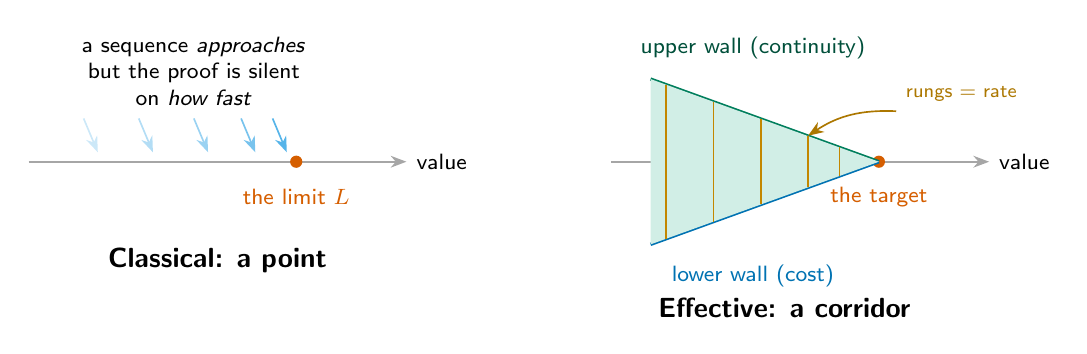
\begin{tikzpicture}[scale=1.0]
  % --- left: the classical point ---
  \begin{scope}
    \draw[arr, gray!70] (-0.2,0) -- (4.6,0) node[right, black]{\footnotesize value};
    \fill[okVerm] (3.2,0) circle (2.2pt);
    \node[okVerm, font=\sffamily\footnotesize] at (3.2,-0.45) {the limit $L$};
    % approaching arrows, never arriving
    \foreach \x/\op in {0.5/30, 1.2/45, 1.9/60, 2.5/80, 2.9/100} {
      \draw[-Stealth, okSky!\op!white, semithick] (\x,0.55) -- (\x+0.18,0.12);
    }
    \node[align=center, font=\sffamily\footnotesize, text=black] at (1.9,1.15)
      {a sequence \emph{approaches}\\ but the proof is silent\\ on \emph{how fast}};
    \node[font=\sffamily\bfseries] at (2.2,-1.25) {Classical: a point};
  \end{scope}
  % --- right: the effective corridor ---
  \begin{scope}[xshift=7.4cm]
    \draw[arr, gray!70] (-0.2,0) -- (4.6,0) node[right, black]{\footnotesize value};
    \fill[okVerm] (3.2,0) circle (2.2pt);
    \node[okVerm, font=\sffamily\footnotesize] at (3.2,-0.45) {the target};
    % shrinking corridor: two converging walls
    \draw[okGreen!80!black, very thick] (0.3,1.05) -- (3.2,0.0);
    \draw[okBlue, very thick] (0.3,-1.05) -- (3.2,0.0);
    \fill[okGreen!18] (0.3,1.05) -- (3.2,0.0) -- (0.3,-1.05) -- cycle;
    % rungs = the ladder = the rate
    \foreach \t in {0.5,1.1,1.7,2.3,2.7} {
      \pgfmathsetmacro{\yy}{1.05*(3.2-\t)/2.9}
      \draw[okOrange!85!black, semithick] (\t,-\yy) -- (\t,\yy);
    }
    % labels placed OUTSIDE the corridor so none sits on an edge, the fill, or a rung
    \node[okGreen!50!black, font=\sffamily\footnotesize, anchor=south] at (1.6,1.18) {upper wall (continuity)};
    \node[okBlue, font=\sffamily\footnotesize, anchor=north] at (1.6,-1.18) {lower wall (cost)};
    \node[okOrange!75!black, font=\sffamily\scriptsize, anchor=west] (rungLbl) at (3.42,0.86) {rungs $=$ rate};
    \draw[okOrange!75!black, -Stealth, semithick] (rungLbl.south west) to[bend right=18] (2.3,0.33);
    \node[font=\sffamily\bfseries] at (2.0,-1.85) {Effective: a corridor};
  \end{scope}
\end{tikzpicture}
\caption{\textbf{The whole idea, before any definition.} Classically a limit is a
\emph{point} that a sequence approaches, with the rate of approach left
unstated~(left). Effectively it is a \emph{corridor}: two walls---one of
continuity, one of cost---closing on the target at a rate carried as data, the
ladder's rungs~(right). The width \emph{is} the object. Read this as a wavepacket
whose error bars are computed, not imposed.}
\label{fig:point-corridor}
\end{figure}

\paragraph{Background.}
The construction synthesizes three frameworks that developed separately. The first
is a point-free ``$\QQ$-free ladder'' that builds compact spaces inductively
without the rational numbers~\citep{iaom_climbing}. The second is a bi-Lipschitz
``corridor'' of golden-ratio bounds that protects a spectral gap from collapse. The
third is the effective functional calculus of Eagle and
McNicholl~\citep{eagle2017computable}, in which every point of a $C^\ast$-algebra is
a stream of finite codes and every theorem returns a program with an explicit
rate~\citep{iaom_spectrum}. Their common thesis is a single statement: a spectrum is
computable \emph{if and only if} it carries a modulus---an explicit positive
certificate that forbids the resolvent from diverging. This paper realizes that
thesis, faithful to its three parts and sharpened in one place, where homotopy type
theory shows the metric was never needed.

% =========================================================================
\section{A measurable construction from Nothing}\label{sec:engine}

\paragraph{Hook.}
Hand a machine a finished number and ask it the rude question: where did you come
from? In the usual telling the question is malformed---$2$ simply \emph{is} an
element of $\NN$, full stop. The Institute's engine refuses the full stop. It
gives every value a \emph{construction trace}: a syntactic record of how the value
was assembled from the empty distinction's two seeds, the void and the mark of the
Laws of Form~\citep{spencerbrown1969laws}. From that trace it reads the value's
history, and from the history it reads \emph{numbers about the number}.

\paragraph{The substrate: dependent type theory.}
The ``void'' and the ``mark'' are not metaphors; they are the primitive type
formers of \emph{dependent type theory}---the empty type that begins with no
element, and the inductive clause that manufactures one structure from another. A
from-Nothing trace is a closed term in this theory, and a value is what that term
evaluates to in a chosen carrier, so provenance is syntactic by construction and the
four observables below are read off the term rather than attached to it. We work in
the homotopy-type-theoretic refinement of this setting~\citep{voevodsky2014univalent},
where a type is read as a space, an equality is a \emph{path}, and univalence makes
equivalent structures equal---so an identification can itself carry computational
content. The machine is \emph{cubical} Agda~\citep{cohen2018cubical,vezzosi2019cubical}:
there univalence is not an axiom one assumes (as in Lean or book HoTT, where the
resulting terms are stuck and compute nothing) but a construction that
\emph{reduces}, which is exactly why the re-entry of \cref{sec:univalence} runs in
the kernel instead of blocking on it. Higher inductive types give the loop, the
quotient, and the colimit as first-class objects rather than encodings, and a
real-cohesive layer~\citep{shulman2018brouwer} supplies the two modalities of
\cref{sec:cohesion}. Every construction in this paper is checked under Agda's
\texttt{--safe} discipline with no postulates; \cref{sec:hott} returns to \emph{why}
each of these ingredients is load-bearing rather than incidental.

\paragraph{Build, then invert.}
The forward map is generative. Choose a system and a trace; obtain a value that
remembers how it was made. The backward map is the engine proper: given a literal,
the \emph{provenance inversion} engine discovers every system in a catalogue that
can host it and reconstructs each system's canonical from-Nothing history. The
central finding of the engine's own development is that the history is genuinely
plural: the value $2$ is a successor ratchet in $\NN$, a ring datum $a+b\theta$ in
the Gaussian integers, a simplest-day cut $\{L\mid R\}$ in Conway's surreal
numbers~\citep{conway2001onag}, and a nested set in the von Neumann
ordinals~\citep{vonneumann1923ordinals}---and these are provably distinct
objects, not one object wearing four labels.

We do not re-derive the engine here; it stands on its own~\citep{iaom_every_number}.
We import one capability: \emph{measurement}. A constructed object is weighed by
four observables, and we will weigh the corridor by the same four.

\begin{definition}[The four observables]\label{def:observables}
For a from-Nothing construction the engine records
\begin{enumerate}[label=(\roman*), nosep, leftmargin=2.2em]
  \item \emph{algebraic behaviour}---which operations close on the carrier;
  \item \emph{provenance cost}---the depth of the construction trace (the Conway
        birthday, for a number; the ladder depth, for the corridor);
  \item \emph{logical entropy}---the Ellerman logical entropy of the history; and
  \item \emph{bare-metal realization}---the value lowered to an interaction-net
        program, ready for a verified reducer whose readback equals its route.
\end{enumerate}
\end{definition}

\paragraph{The one observable that does the philosophical work.}
The third is the surprising one. \emph{Logical entropy}~\citep{ellerman2009counting,
ellerman2018logical} measures the distinction content of a partition: it is the
probability that two independent draws land in different blocks,
\begin{equation}\label{eq:logical-entropy}
  \Llog(\pi) \;=\; 1 - \sum_{B \in \pi} \Big(\tfrac{|B|}{|U|}\Big)^{2}
  \;=\; \frac{\#\{\text{ordered pairs separated by }\pi\}}{|U|^{2}},
\end{equation}
the Gini--Simpson index read as a count of \emph{distinctions made}. It is not
Shannon entropy in disguise; it is the older, more primitive notion---how much a
structure tells apart---and it is exactly additive over the making of
distinctions. The engine computes it, not tabulates it: the number $2$ has
logical entropy $4/9$ in $\NN$, $36/49$ in the Gaussian integers, $12/25$ in the
surreals. Same value, different histories, \emph{different measurable distinction
content}.

We flag this now because the corridor's $H^1$ screen
(\cref{sec:screen}) will turn out to carry positive logical entropy of exactly
this kind. The cohomological obstruction that Veselov's proposal predicted---a
class locally trivial but globally not---is, when measured, a distinction the
boundary makes and no deformation unmakes. The engine's currency and the
corridor's obstruction are the same coin.

\paragraph{The catalogue and its complexity.}
The plurality is not a handful of special cases; it is a \emph{catalogue}. From the
same two seeds the engine climbs a ladder of number systems---each a genuine
algebraic structure with its own from-Nothing history, and therefore its own
complexity profile---topped by the surreal numbers, the universal rung on which
every value of every lower system is born on a definite day~\citep{conway2001onag,
iaom_every_number}. \Cref{fig:numladder} draws the ladder; \cref{tab:catalogue} weighs a
representative element of each system by the same four observables we will apply to
the corridor. Two readings carry into the rest of the paper. First, the
\emph{provenance cost}---the Conway birthday---is intrinsic, not a matter of
notation: the integer $n$ is born on day $n$, while the golden ratio, the corridor's
own value, is born on day $\omega$, the first transfinite day, the same $\omega$
where the corridor's forced golden modulus reappears in \cref{sec:modulus}. Second,
the \emph{logical entropy} of one fixed value depends on the system that hosts
it---$2$ carries $4/9$ in $\NN$, $36/49$ in the Gaussian integers, and $12/25$ in
the surreals---so ``the number $2$'' names not one object but a family of measurably
distinct histories. The corridor, weighed in \cref{sec:synthesis}, enters the same
catalogue as its own row.

\begin{table}[t]
\centering
\caption{\textbf{The catalogue, weighed.} A representative element of each number
system the engine builds from the two seeds, read by four observables: its
from-Nothing history, the algebra that closes on it, its provenance cost (the Conway
birthday of the witness), and the logical entropy of the witness where the engine
has computed it. The corridor (last row) enters the same catalogue; ``\,---\,''
marks an observable not computed here.}
\label{tab:catalogue}
\small
\begin{tabular}{@{}llllc@{}}
\toprule
\textbf{system} & \textbf{from-Nothing history} & \textbf{closes under} & \textbf{birthday} & $\bm{\Llog}$ \\
\midrule
$\NN$                  & $\mathsf{succ}^{n}\,\mathbf 0$            & commutative semiring          & $n$              & $4/9$ \\
$\ZZ$                  & $\pm\,\mathsf{succ}^{n}\,\mathbf 0$       & commutative ring              & $n$              & --- \\
dyadic $\QQ$           & mediant cuts                              & field                         & cut depth        & --- \\
Gaussian $\ZZ[i]$      & $a \oplus b\,\theta,\ \theta^{2}{=}{-}1$  & ring with conjugation         & $n$              & $36/49$ \\
surreals               & $\{L \mid R\}$, day-bounded               & ordered field (universal)     & the day itself   & $12/25$ \\
von Neumann ordinals   & nested sets                               & well-order                    & rank             & --- \\
staged $\RR$           & modulus program                           & complete ordered field        & $\omega$ (at $\varphi$) & --- \\
\midrule
\textbf{the corridor}  & golden modulus ladder                     & two cohesion walls, no metric & golden depth $D$ & $\bm{1/2}$ \\
\bottomrule
\end{tabular}
\end{table}

\begin{figure}[t]
\centering
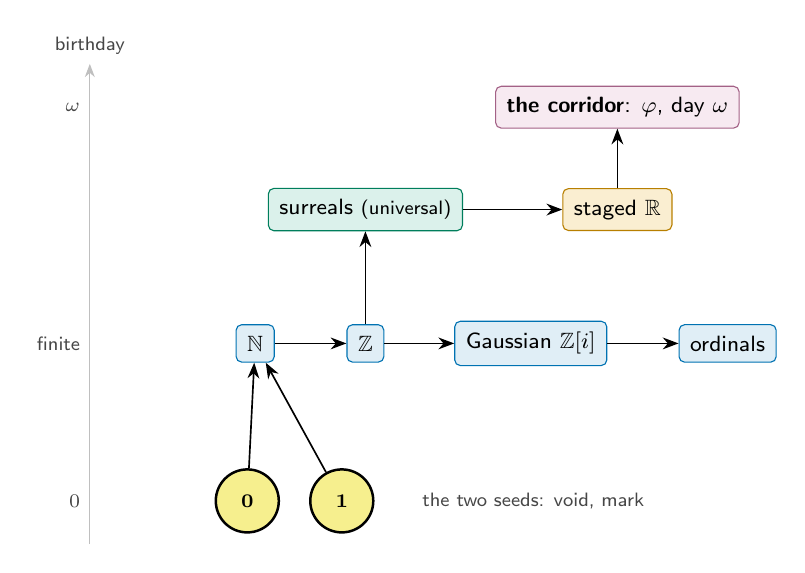
\begin{tikzpicture}[every node/.style={font=\sffamily\footnotesize}]
  % birthday axis
  \draw[-Stealth, gray!50] (-0.5,-0.55) -- (-0.5,5.55) node[above, font=\sffamily\scriptsize, text=gray!55!black]{birthday};
  \node[font=\sffamily\scriptsize, text=gray!55!black, left] at (-0.5,0.0) {$0$};
  \node[font=\sffamily\scriptsize, text=gray!55!black, left] at (-0.5,2.0) {finite};
  \node[font=\sffamily\scriptsize, text=gray!55!black, left] at (-0.5,5.0) {$\omega$};
  % seeds
  \node[seed] (zero) at (1.5,0) {$\mathbf 0$};
  \node[seed] (one)  at (2.7,0) {$\mathbf 1$};
  \node[font=\sffamily\scriptsize, text=gray!55!black, anchor=west] at (3.6,0) {the two seeds: void, mark};
  % finite rung
  \node[boxBlue] (nat)   at (1.6,2.0) {$\NN$};
  \node[boxBlue] (int)   at (3.0,2.0) {$\ZZ$};
  \node[boxBlue] (gauss) at (5.1,2.0) {Gaussian $\ZZ[i]$};
  \node[boxBlue] (ord)   at (7.6,2.0) {ordinals};
  % transfinite rung
  \node[boxGreen]  (sur)  at (3.0,3.7) {surreals {\scriptsize(universal)}};
  \node[boxOrange] (real) at (6.2,3.7) {staged $\RR$};
  % the corridor, highlighted
  \node[boxPurple] (cor)  at (6.2,5.0) {\textbf{the corridor}: $\varphi$, day $\omega$};
  % climbing arrows
  \draw[arr] (zero) -- (nat); \draw[arr] (one) -- (nat);
  \draw[arr] (nat) -- (int); \draw[arr] (int) -- (gauss); \draw[arr] (gauss) -- (ord);
  \draw[arr] (int) -- (sur); \draw[arr] (sur) -- (real); \draw[arr] (real) -- (cor);
\end{tikzpicture}
\caption{\textbf{The ladder of number systems.} From the two seeds the engine builds
a catalogue of genuine number systems, each born on a definite day: a finite rung
($\NN$, $\ZZ$, the Gaussian integers, the ordinals), then the surreals---the
universal rung on which every lower value is born on a definite day---and the staged
reals. The golden value $\varphi$ that the corridor realizes is born on day
$\omega$, the first transfinite day; the corridor (\cref{sec:synthesis}) is its
effective, metric-free presentation.}
\label{fig:numladder}
\end{figure}

\begin{figure}[t]
\centering
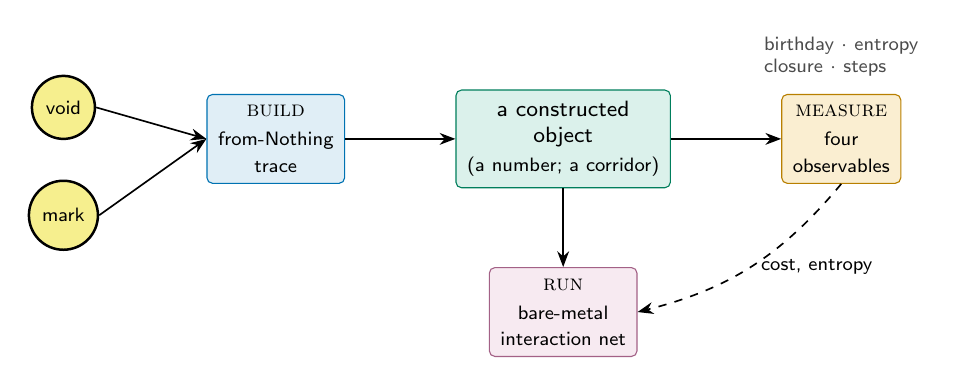
\begin{tikzpicture}[node distance=8mm]
  \node[seed] (void) {void};
  \node[seed, below=5mm of void] (mark) {mark};
  \node[boxBlue, right=14mm of void, yshift=-4mm] (build) {\textsc{build}\\[1pt]\scriptsize from-Nothing\\\scriptsize trace};
  \node[boxGreen, right=14mm of build] (obj) {a constructed\\object\\[1pt]\scriptsize (a number; a corridor)};
  \node[boxOrange, right=14mm of obj] (meas) {\textsc{measure}\\[1pt]\scriptsize four\\\scriptsize observables};
  \node[boxPurple, below=10mm of obj] (metal) {\textsc{run}\\[1pt]\scriptsize bare-metal\\\scriptsize interaction net};
  \draw[arr] (void.east) -- (build.west);
  \draw[arr] (mark.east) -- (build.west);
  \draw[arr] (build) -- (obj);
  \draw[arr] (obj) -- (meas);
  \draw[arr] (obj) -- (metal);
  \draw[arrd] (meas.south) to[bend left=18] node[right, font=\sffamily\scriptsize]{cost, entropy} (metal.east);
  \node[font=\sffamily\scriptsize, text=gray!60!black, align=left, above=1mm of meas]
    {birthday $\cdot$ entropy\\ closure $\cdot$ steps};
\end{tikzpicture}
\caption{\textbf{The engine in one line.} Every object is built from the empty
distinction's two seeds, \emph{measured} by four observables (one of them logical
entropy), and lowered to (the engine runs) a bare-metal interaction net. This paper
feeds one new object---the effective corridor---through the same stations, reaching
the third as a lowering (\cref{sec:metal}).}
\label{fig:engine}
\end{figure}

\paragraph{What we inherit, precisely.}
From the engine we take the discipline that an object is not finished when it
type-checks but when it \emph{reaches executable bare-metal form and is measured}.
From the from-Nothing
companion we take the starting point literally: our corridor will be built from
the same two seeds---the void and the mark---and its first nontrivial structure,
the re-entry of \cref{sec:univalence}, is the Laws-of-Form crossing itself. The
remainder of the paper is the corridor's passage through the three stations of
\cref{fig:engine}: it is built (\cref{sec:cohesion,sec:univalence,sec:modulus,%
sec:screen}), bound into one object (\cref{sec:synthesis}), measured, and run
(\cref{sec:metal}).

% =========================================================================
\section{Two walls, intrinsically}\label{sec:cohesion}

\paragraph{Hook.}
Stand inside the corridor and put a hand on each wall. The two walls feel
different. The upper wall is smooth: slide along it and nothing snags, because it
records only \emph{nearness}---whether two states are connected, not whether they
are equal. The lower wall is rough: it records \emph{difference}---it refuses to
let two distinct states be confused, and that refusal is where the constructive
work, the cost, accumulates. The original proposal asked for these two walls and
proposed to separate them with a metric, a bi-Lipschitz pair of golden-ratio
bounds. Homotopy type theory offers something cleaner: the two walls are two
\emph{modalities}, and they are different functors with no metric in sight.

\paragraph{The setting.}
In real-cohesive homotopy type theory~\citep{shulman2018brouwer} a type may carry
\emph{cohesion}---a primitive notion of which points hang together---exposed
through an adjoint string of modalities
\begin{equation}\label{eq:cohesion-adjoint}
  \shapeM \;\dashv\; \flatM \;\dashv\; \sharpM,
\end{equation}
the \emph{shape}, \emph{flat}, and \emph{sharp}. Shape $\shapeM A$ contracts each
cohesive blob to a point: it is the homotopy type underlying $A$, blind to
everything but connectedness. Flat $\flatM A$ does the opposite: it keeps the
points and forgets the cohesion, exposing $A$'s underlying \emph{discrete}
collection. In one slogan: $\shapeM$ is topology, $\flatM$ is
distinguishability. The corridor's continuity wall is the shape; its cost wall is
the flat. That the two walls are genuinely different is then the assertion that
\emph{$\shapeM$ and $\flatM$ are different functors}---and this is exactly what a
metric-free model must, and here does, make true.

\paragraph{A model where the walls separate.}
We realize cohesion finitely. A cohesive type is a set $A$ equipped with a
prop-valued equivalence relation $\sim$ (``in the same connected piece''); a
morphism preserves $\sim$. The four cohesive coreflections are the standard ones,
\begin{equation}\label{eq:cohesion-modalities}
  \PiZero A = A/{\sim}, \qquad
  \shapeM A = \Disc(\PiZero A), \qquad
  \flatM A = \Disc(\Gam A), \qquad
  \sharpM A = \coDisc(\Gam A),
\end{equation}
where $\Gam$ forgets $\sim$, $\Disc$ equips a set with equality-cohesion, and
$\coDisc$ with total cohesion. The shape collapses each connected piece to a point
and then makes the result discrete; the flat keeps every point and severs every
tie.

\begin{theorem}[The shape--flat adjunction is genuine]\label{thm:shapeflat}
For all cohesive $A,B$ there is an isomorphism, natural in both,
\begin{equation}\label{eq:shapeflat-iso}
  \Hom(\shapeM A,\,B)\;\cong\;\Hom(A,\,\flatM B),
\end{equation}
and it is \emph{not} the identity: it is the universal property of the
set-quotient, sending a map out of the component-set to the map on points that is
constant on $\sim$-classes.
\end{theorem}

\noindent\emph{Picture.} A map from the collapsed corridor (its components) to a
target is the same as a map from the corridor that cannot tell two endpoints in
the same component apart. \emph{Statement.} \cref{eq:shapeflat-iso}.
\emph{Meaning.} The adjunction is the content of cohesion; realizing it as the
quotient universal property---rather than as $\Hom(A,B)=\Hom(A,B)$, the empty
identity a degenerate model would offer---is what makes the two walls do work.
\emph{Proof.} The forgetful-to-quotient transposition is the set-quotient
recursor; left and right inverses are the quotient's $\beta$- and
$\eta$-rules. The construction is kernel-checked under \texttt{-{}-cubical
-{}-safe} with no postulates.\hfill$\square$

\begin{theorem}[The walls are different functors]\label{thm:shapenotflat}
Let $\Bd$ be the corridor's interval: the two-element boundary with \emph{total}
cohesion (the two endpoints connected). Then
\begin{equation}\label{eq:shape-collapses}
  \isContr\big(\Carrier(\shapeM \Bd)\big)
  \qquad\text{while}\qquad
  \neg\,\isContr\big(\Carrier(\flatM \Bd)\big),
\end{equation}
and consequently $\Carrier(\shapeM \Bd)\equiv\Carrier(\flatM \Bd)$ is
contradictory: $\shapeM\neq\flatM$.
\end{theorem}

\noindent\emph{Picture.} Shape squeezes the corridor's two endpoints into one
point (it is connected); flat keeps them two (they are distinct). \emph{Statement.}
\cref{eq:shape-collapses}. \emph{Meaning.} Topology cannot see the endpoints
apart; distinguishability can. This is the corridor's two walls, separated by a
\emph{theorem about modalities}, with no metric: the one awkward import of the
original proposal---a bi-Lipschitz constant living between a point-free ontology
and a metric estimate---is discharged and then deleted. \emph{Proof.} The shape
is the quotient of a two-point set by the total relation, which is the interval
type, contractible; the flat is the two-point set with equality, where the two
points are apart by the discreteness of $\mathbb{2}$. A transport of
contractibility along a putative identification of carriers would force the two
boundary points equal, contradiction.\hfill$\square$

\begin{figure}[t]
\centering
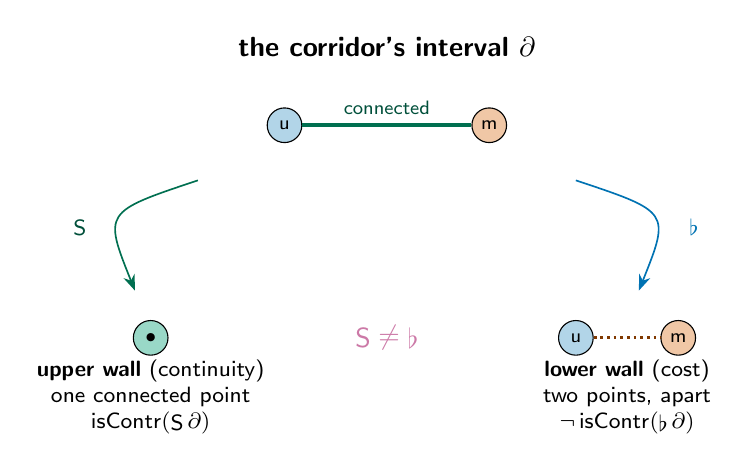
\begin{tikzpicture}[scale=1.0]
  % the boundary interval
  \node[font=\sffamily\bfseries] at (0,1.7) {the corridor's interval $\Bd$};
  \node[pt, fill=okBlue!30] (u) at (-1.3,0.7) {$\unmk$};
  \node[pt, fill=okVerm!35] (m) at (1.3,0.7) {$\mkd$};
  \draw[okGreen!70!black, line width=1.4pt] (u) -- (m) node[midway, above, font=\sffamily\scriptsize, text=okGreen!50!black]{connected};
  % shape arrow
  \draw[arr, okGreen!70!black] (-2.4,0.0) .. controls (-3.6,-0.4) .. (-3.2,-1.4);
  \node[font=\sffamily\footnotesize, text=okGreen!50!black] at (-3.9,-0.6) {$\shapeM$};
  \node[pt, fill=okGreen!40] (s) at (-3.0,-2.0) {$\bullet$};
  \node[font=\sffamily\footnotesize, align=center] at (-3.0,-2.75)
    {\textbf{upper wall} (continuity)\\ one connected point\\ $\isContr(\shapeM\Bd)$};
  % flat arrow
  \draw[arr, okBlue] (2.4,0.0) .. controls (3.6,-0.4) .. (3.2,-1.4);
  \node[font=\sffamily\footnotesize, text=okBlue] at (3.9,-0.6) {$\flatM$};
  \node[pt, fill=okBlue!30] (fu) at (2.4,-2.0) {$\unmk$};
  \node[pt, fill=okVerm!35] (fm) at (3.7,-2.0) {$\mkd$};
  \draw[okVerm!60!black, line width=1.0pt, dash pattern=on 1pt off 1.4pt] (fu) -- (fm);
  \node[font=\sffamily\footnotesize, align=center] at (3.05,-2.75)
    {\textbf{lower wall} (cost)\\ two points, apart\\ $\neg\,\isContr(\flatM\Bd)$};
  \node[font=\sffamily\bfseries, text=okPurple] at (0,-2.0) {$\shapeM\neq\flatM$};
\end{tikzpicture}
\caption{\textbf{The two walls, separated without a metric.} The shape modality
$\shapeM$ collapses the corridor's connected interval to a single point---the
continuity wall sees only nearness. The flat modality $\flatM$ keeps the two
endpoints apart---the cost wall sees difference. That these are different functors
(\cref{thm:shapenotflat}) is the corridor's structure stated in pure cohesion.}
\label{fig:two-walls}
\end{figure}

\paragraph{Why this needs homotopy type theory.}
A first attempt at a cohesive corridor over an ordinary type fails for a sharp
reason. If the ``type'' is a bare set and morphisms are bare functions, then a
left adjoint $\shapeM$ satisfying $\shapeM\shapeM\cong\shapeM$ is forced by a
copower argument to be either the identity or the constant-empty functor---there
is no room for a nontrivial shape. The walls collapse onto each other. Cohesion is
exactly the extra structure that breaks this: by remembering which points hang
together, the type lets $\shapeM$ quotient and $\flatM$ keep, and
\cref{thm:shapenotflat} becomes available. Homotopy type theory is where this
structure is native and where the modalities come with their adjunctions already
proved. The metric in the original proposal was a stand-in for a separation that
the type system supplies directly.

% =========================================================================
\section{The square root of re-entry}\label{sec:univalence}

\paragraph{Hook.}
Draw a mark. Draw a mark around the mark. In George Spencer-Brown's calculus the
second act is \emph{re-entry}: the form crosses its own boundary and comes back
changed~\citep{spencerbrown1969laws}. Re-entry is an operation that, applied
twice, returns you to where you started while sending each state to its
opposite---a reflection, an involution, the discrete shadow of multiplication by
$-1$. The corridor's target is the fixed object of this re-entry, and to build it
honestly we need the re-entry to be a genuine \emph{identification} of the
boundary with itself, not a function that happens to swap two labels. This is the
one place the construction stands or falls on \emph{univalence}---and on
univalence of the kind that computes.

\paragraph{The crossing.}
Let $\Bd=\{\unmk,\mkd\}$ be the boundary, and let $\cross\colon\Bd\to\Bd$ be the
Laws-of-Form crossing, $\cross(\unmk)=\mkd$, $\cross(\mkd)=\unmk$. It is its own
inverse,
\begin{equation}\label{eq:cross-involution}
  \cross\circ\cross = \mathrm{id}_{\Bd},
\end{equation}
so $\cross$ is the period-two re-entry: the half-turn whose square is the full
turn. (Its own square root---the quarter-turn, the genuine $\sqrt{-1}$---is the
phase that the Institute's Euler-witness construction pins as the third truth
value; here we need only the half-turn.) As a map of finite sets $\cross$ is an
equivalence $\Bd\simeq\Bd$.

\paragraph{The identification that computes.}
Univalence~\citep{voevodsky2014univalent} turns an equivalence into a path of
types. In the \emph{cubical} setting~\citep{cohen2018cubical,vezzosi2019cubical}
this path is not an axiom one assumes but a construction that \emph{reduces}: the
glued path $\ua(\cross)\colon\Bd\equiv\Bd$ is built from Glue, and transport along
it computes.

\begin{theorem}[Re-entry transports, and is not trivial]\label{thm:ua}
The univalence path of the crossing satisfies
\begin{equation}\label{eq:ua-transport}
  \transport^{\,\ua(\cross)}(\unmk) \;=\; \mkd,
\end{equation}
which reduces to $\mkd$ in the kernel, and consequently the path is genuinely
nontrivial:
\begin{equation}\label{eq:ua-nontrivial}
  \big(\ua(\cross)\equiv\mathrm{refl}_{\Bd}\big)\;\to\;\bot.
\end{equation}
\end{theorem}

\noindent\emph{Picture.} Carry a state along the re-entry path and it comes back
flipped---unmarked becomes marked---so the path cannot be the trivial loop.
\emph{Statement.} \cref{eq:ua-transport,eq:ua-nontrivial}. \emph{Meaning.} In a
physicist's reading the boundary is a two-level system and the re-entry is a
reflection acting on it; \cref{eq:ua-transport} is that reflection \emph{realized
as transport}, and \cref{eq:ua-nontrivial} certifies it is not the identity---the
re-entry does real work. \emph{Proof.} The cubical Glue construction makes
$\transport^{\,\ua(\cross)}$ definitionally the forward map of $\cross$, so
\cref{eq:ua-transport} holds by reflexivity in the kernel. Were the path
reflexive, transport along it would fix $\unmk$; but it sends $\unmk$ to $\mkd$,
and $\mkd\neq\unmk$ by discreteness of $\Bd$, giving \cref{eq:ua-nontrivial}.
\hfill$\square$

\begin{figure}[t]
\centering
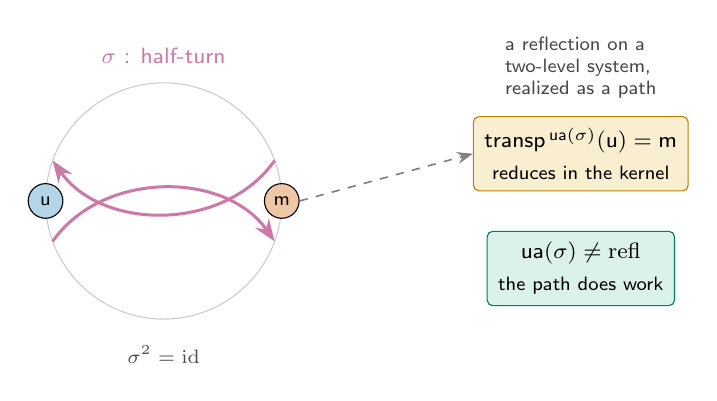
\begin{tikzpicture}[scale=1.0]
  % two-level system, the half-turn
  \draw[gray!40] (0,0) circle (1.5);
  \node[pt, fill=okBlue!30] (u) at (180:1.5) {$\unmk$};
  \node[pt, fill=okVerm!35] (m) at (0:1.5) {$\mkd$};
  \draw[arr, okPurple, line width=1.1pt] (200:1.5) to[bend left=55] (340:1.5);
  \draw[arr, okPurple, line width=1.1pt] (20:1.5) to[bend left=55] (160:1.5);
  \node[okPurple, font=\sffamily\footnotesize] at (0,1.84) {$\cross$ : half-turn};
  \node[font=\sffamily\scriptsize, text=gray!60!black] at (0,-1.95) {$\cross^2=\mathrm{id}$};
  % transport box
  \node[boxOrange, right=22mm of m, yshift=6mm] (tr)
    {$\transport^{\,\ua(\cross)}(\unmk)=\mkd$\\[2pt]\scriptsize reduces in the kernel};
  \node[boxGreen, below=5mm of tr] (nt)
    {$\ua(\cross)\neq\mathrm{refl}$\\[2pt]\scriptsize the path does work};
  \draw[arrd, gray] (m.east) -- (tr.west);
  \node[font=\sffamily\scriptsize, align=left, text=gray!55!black, above=1mm of tr]
    {a reflection on a\\ two-level system,\\ realized as a path};
\end{tikzpicture}
\caption{\textbf{Re-entry as a computing identification.} The crossing $\cross$ is
the half-turn on the two-state boundary, an involution ($\cross^2=\mathrm{id}$).
Univalence makes it a path of types whose transport \emph{reduces}: carrying
$\unmk$ along it yields $\mkd$ (\cref{eq:ua-transport}), so the path is genuinely
nontrivial (\cref{eq:ua-nontrivial}). In Lean this term is stuck on the univalence
axiom; in cubical type theory it runs.}
\label{fig:crossing}
\end{figure}

\paragraph{Why this needs homotopy type theory---and why cubical.}
Outside univalent foundations, ``the boundary is identified with itself by the
re-entry'' is either false (the two-element set is not equal to itself in any
nontrivial way) or a bare axiom with no computational content. Univalence makes
the statement true and meaningful; \emph{cubical} univalence makes it
\emph{compute}, so \cref{eq:ua-transport} is a reduction rather than a promise.
The same term, transcribed into a kernel without a computing univalence, is
provably stuck---it cannot take a step---which is precisely the symptom that the
content has been lost. The corridor's target is reached by a path that runs, and
that running is later what lets the whole object lower to bare metal. This is the
sharpest single illustration in the paper of why the choice of foundation is not
cosmetic.

% =========================================================================
\section{The ladder is the rate}\label{sec:modulus}

\paragraph{Hook.}
A modulus is a promise with a deadline. ``The sequence converges'' is a promise;
``to within $2^{-k}$, look past term $\modulus(k)$'' is the same promise with a
deadline attached, and the deadline is the whole difference between a number you
believe in and a number you can run. Effective functional analysis is built on
this move: in Eagle and McNicholl's calculus every point of a $C^\ast$-algebra is
a stream of finite codes and every norm is an oracle with a
rate~\citep{eagle2017computable}. Veselov's proposal sharpened it to an
equivalence: a spectrum is computable \emph{iff} it has a modulus, a positive
certificate $c>0$ that forbids the resolvent from diverging---geometrically, a
lower wall that never lets the corridor's gap collapse to the ``syntactic
horizon,'' the decay filter where everything has gone to zero. We make the
modulus, and we make it \emph{forced}.

\paragraph{The golden, $\QQ$-free ladder.}
We refuse the rational numbers and zero alike, exactly as the point-free ladder
demands~\citep{iaom_climbing}. The scaffold is the golden one: the Fibonacci
numbers $\fib_n$ (with $\fib_1=\fib_2=1$, $\fib_{n+2}=\fib_{n+1}+\fib_n$), whose
ratios climb to $\varphi$ and whose growth is the Pisot self-similarity of
$\Zphi$~\citep{zeckendorf1972representation}. Rung $n$ of the corridor carries a
bracket of \emph{denominator}
\begin{equation}\label{eq:width}
  w(n) \;=\; \fib_{n+2} \;=\; 1,2,3,5,8,\dots
\end{equation}
a larger denominator meaning a narrower bracket. The modulus reads a precision
demand $D$ and returns a rung; the content is that it can, and that no constant
can.

\begin{theorem}[Soundness: the ladder reaches any precision]\label{thm:modsound}
The golden growth dominates the linear demand,
\begin{equation}\label{eq:fib-lower}
  \fib_{n+2}\;\ge\; n+1 \qquad(\text{for all }n),
\end{equation}
so the modulus $\modulus(D)=D$ achieves the demanded denominator:
$D\le w(\modulus(D))$.
\end{theorem}

\noindent\emph{Picture.} Ask for precision $D$; walk $D$ rungs down the ladder;
the bracket there is at least as fine as you asked. \emph{Statement.}
\cref{eq:fib-lower}. \emph{Meaning.} The certificate $c>0$ exists and is
explicit---this is the resolvent-non-divergence guarantee, the lower wall holding.
\emph{Proof.} Induction: $\fib_{n+3}=\fib_{n+2}+\fib_{n+1}\ge(n+1)+1$ since
$\fib_{n+1}\ge1$. Kernel-checked over $\NN$ with no real-number machinery, hence
genuinely $\QQ$-free.\hfill$\square$

\begin{theorem}[The rate is forced: no constant modulus]\label{thm:modforced}
The ladder strictly narrows, $w(n)<w(n+1)$, and consequently for every fixed rung
$c$ there is a precision it cannot meet:
\begin{equation}\label{eq:no-constant}
  \forall\, c.\;\exists\, D.\; w(c) < D .
\end{equation}
No constant function is a sound modulus.
\end{theorem}

\noindent\emph{Picture.} Stop at any fixed rung and there is always a finer
precision than that rung delivers; you must keep walking. \emph{Statement.}
\cref{eq:no-constant}. \emph{Meaning.} This is the heart of ``the ladder is the
rate.'' The rate is not a parameter one may set to a constant and forget; the
structure refuses it. The proposal's physical reading makes the analogy precise:
a UV-divergence is a gap that stops shrinking, and in this formal model such a gap
\emph{is} a constant modulus, so \cref{thm:modforced} is the formal impossibility
of one. We claim the formal theorem; the physical interpretation is Veselov's, and
the point is that it is now auditable rather than asserted. The
upper bound of the original bi-Lipschitz pair guarded against chaos; this lower,
forced bound is the one that carries the ontology, and it survives the deletion of
the metric. \emph{Proof.} Take $D=w(c)+1$; then $w(c)<D$ by the irreflexivity of
$<$. Strict narrowing is positivity of the Fibonacci increment.\hfill$\square$

\begin{figure}[t]
\centering
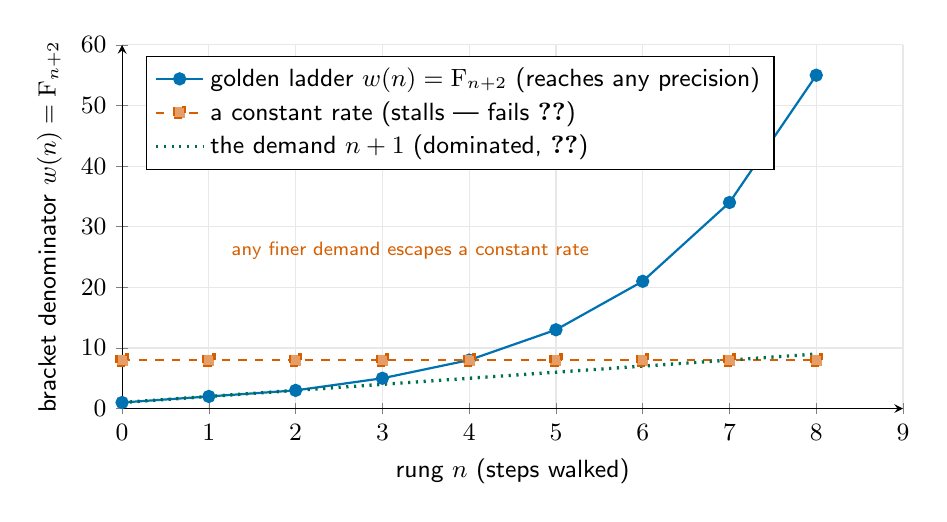
\begin{tikzpicture}
\begin{axis}[
  width=11.5cm, height=6.2cm,
  xlabel={rung $n$ (steps walked)},
  ylabel={bracket denominator $w(n)=\fib_{n+2}$},
  xmin=0, xmax=9, ymin=0, ymax=60,
  xtick={0,1,...,9}, ytick={0,10,...,60},
  legend pos=north west, legend cell align=left,
  grid=both, grid style={gray!18}, axis lines=left,
  every axis plot/.append style={thick},
]
  % golden ladder
  \addplot[okBlue, mark=*, mark options={fill=okBlue}]
    coordinates {(0,1)(1,2)(2,3)(3,5)(4,8)(5,13)(6,21)(7,34)(8,55)};
  \addlegendentry{golden ladder $w(n)=\fib_{n+2}$ (reaches any precision)}
  % a constant modulus
  \addplot[okVerm, dashed, mark=square*, mark options={fill=okVerm!60}]
    coordinates {(0,8)(1,8)(2,8)(3,8)(4,8)(5,8)(6,8)(7,8)(8,8)};
  \addlegendentry{a constant rate (stalls --- fails \cref{thm:modforced})}
  % linear demand floor
  \addplot[okGreen!70!black, dotted, very thick]
    coordinates {(0,1)(8,9)};
  \addlegendentry{the demand $n+1$ (dominated, \cref{eq:fib-lower})}
  \node[okVerm, font=\sffamily\scriptsize, anchor=west] at (axis cs:1.15,26)
    {any finer demand escapes a constant rate};
\end{axis}
\end{tikzpicture}
\caption{\textbf{Why the ladder must be the rate.} The golden bracket
$w(n)=\fib_{n+2}$ (blue) overtakes any linear precision demand
(\cref{eq:fib-lower}) and strictly narrows forever. A \emph{constant} rate (red,
dashed) stalls at a fixed fineness and is beaten by some demand
(\cref{thm:modforced})---the formal shadow of a UV-divergence, here proved
impossible. The convergence cannot be faked.}
\label{fig:ladder}
\end{figure}

% =========================================================================
\section{Approximants and a topological screen}\label{sec:screen}

\paragraph{Hook.}
Two questions remained in the proposal, and they are the two that a physicist
cares about most. Can the continuous object be reached by \emph{finite}
approximants, so that a computation actually terminates at each stage? And does
the act of approximating leave a \emph{residue}---an obstruction that is invisible
locally but real globally, the kind of thing that, in a gauge theory, becomes a
flux or a charge? The answer to both is yes, and the second answer is where the
corridor's measurement closes the loop with the engine.

\paragraph{Finite approximants: the $\Zphi$ colimit.}
Following the proposal's Part~II we approximate over the golden ring $\Zphi$ by a
sequence of finite stages whose sizes are the ladder denominators. Stage $n$ is
the finite set
\begin{equation}\label{eq:af-stage}
  \mathrm{St}(n) \;=\; \{\,k : k < w(n)\,\},
\end{equation}
included into stage $n{+}1$ by the inclusion that keeps each point's value, and the
effective object is the sequential colimit
\begin{equation}\label{eq:af-colim}
  \mathrm{St}_\infty \;=\; \colim\big(\mathrm{St}(0)\hookrightarrow
  \mathrm{St}(1)\hookrightarrow\cdots\big),
\end{equation}
a higher inductive type with point and path constructors.

\begin{theorem}[The colimit genuinely grows]\label{thm:af}
Each inclusion is non-surjective: the value $w(n)$ first appears at stage $n{+}1$
and is reached by no point of stage $n$,
\begin{equation}\label{eq:nonsurj}
  \big(\,\mathrm{fst}(q) \equiv w(n)\,\big)\to\bot
  \qquad\text{for every } q\in\mathrm{St}(n).
\end{equation}
Hence no finite stage exhausts $\mathrm{St}_\infty$.
\end{theorem}

\noindent\emph{Picture.} Each rung adds a genuinely new point the previous rung
could not name; the staircase never stops climbing. \emph{Statement.}
\cref{eq:nonsurj}. \emph{Meaning.} This is the combinatorial skeleton of an
approximately-finite approximation---a Bratteli tower of finite stages with proper
inclusions, the shape the dimension data of an AF $C^\ast$-algebra would carry---so
the continuous object is the honest limit of finite data, and a degenerate ``AF''
colimit whose maps were equivalences (a tower that secretly stopped) is excluded.
We claim the skeleton here; \cref{sec:formalization} refines it to the
finite-dimensional matrix $\ast$-algebras, leaving the operator-norm limit as the
one part still open. \emph{Proof.} Every point of stage $n$ has value strictly
below $w(n)$; the inclusion preserves value; so the fresh value $w(n)$ is missed.
\hfill$\square$

\paragraph{The global residue: an $H^1$ logical-entropy screen.}
Part~III of the proposal predicted that the ``infinite swarm'' of a truncated
mode---the observer as a screening boundary---would be a cochain \emph{locally a
coboundary but globally a nontrivial $H^1$ class}. The re-entry loop of
\cref{sec:univalence} is exactly the space that hosts such a class. Take the
circle $S^1$ (one vertex, one edge that is a loop) with $\bbtwo$ coefficients; the
coboundary of a $0$-cochain along the loop is $\delta^0 f = f\oplus f$.

\begin{theorem}[Locally a coboundary, globally nontrivial---and it makes a distinction]
\label{thm:h1}
On the re-entry loop the coboundary vanishes,
\begin{equation}\label{eq:delta-vanish}
  \delta^0 f \;=\; f\oplus f \;=\; 0 \qquad(\text{for all } f),
\end{equation}
so every $1$-cochain is closed; yet the loop class $\omega=1$ is not a coboundary,
\begin{equation}\label{eq:not-exact}
  \big(\delta^0 f \equiv 1\big)\to\bot,
  \qquad\text{i.e.}\qquad H^1(S^1;\bbtwo)\cong\bbtwo\neq 0,
\end{equation}
and this nonzero class carries strictly positive logical entropy,
$\Llog(\omega{=}1)=\tfrac12>0$, while a coboundary screens to zero.
\end{theorem}

\noindent\emph{Picture.} Around the loop the obstruction cancels at every point
yet refuses to cancel overall---a charge you cannot see locally but cannot deform
away. \emph{Statement.} \cref{eq:delta-vanish,eq:not-exact}. \emph{Meaning.} This
is the proposal's screening boundary, realized: a flux through the re-entry loop,
of order two, exactly the cohomological signature predicted for the observer. And
crucially it is \emph{measured}: by \cref{eq:logical-entropy} the nonzero class
separates the two boundary states---two ordered distinctions out of four pairs,
logical entropy $\tfrac12$---the very same logical-entropy currency the engine
reads off a number's provenance (\cref{sec:engine}). The topology of the
obstruction and the distinction content of the boundary are one quantity.
\emph{Proof.} $f\oplus f=0$ by case analysis on $\bbtwo$; if a coboundary equalled
$1$ then $0\equiv1$, impossible; the distinction count of the discrete partition
of $\{\unmk,\mkd\}$ is $2$, giving $\Llog=\tfrac{2}{4}$.\hfill$\square$

\begin{figure}[t]
\centering
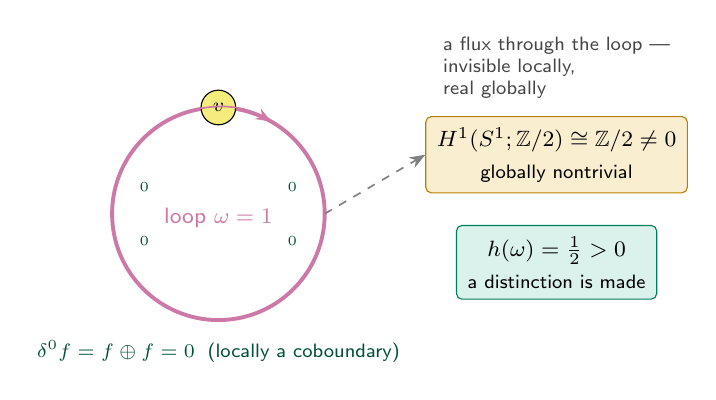
\begin{tikzpicture}[scale=1.0]
  % the loop with vanishing local coboundary but nontrivial class
  \draw[okPurple, line width=1.4pt] (0,0) circle (1.35);
  \node[pt, fill=okYellow!70] (v) at (90:1.35) {$v$};
  \draw[arr, okPurple] (130:1.35) arc (130:60:1.35);
  \node[okPurple, font=\sffamily\footnotesize] at (0,-0.05) {loop $\omega=1$};
  \node[font=\sffamily\scriptsize, text=okGreen!50!black] at (0,-1.75)
    {$\delta^0 f=f\oplus f=0$ \;(locally a coboundary)};
  % local cancellation markers
  \foreach \a in {20,160,200,340} {
     \node[font=\sffamily\tiny, text=okGreen!50!black] at (\a:1.0) {$0$};
  }
  % the global class + entropy
  \node[boxOrange, right=24mm of v, yshift=-6mm] (cls)
    {$H^1(S^1;\bbtwo)\cong\bbtwo\neq0$\\[2pt]\scriptsize globally nontrivial};
  \node[boxGreen, below=4mm of cls] (ent)
    {$\Llog(\omega)=\tfrac12>0$\\[2pt]\scriptsize a distinction is made};
  \draw[arrd, gray] (0:1.35) -- (cls.west);
  \node[font=\sffamily\scriptsize, align=left, text=gray!55!black, above=1mm of cls]
    {a flux through the loop ---\\ invisible locally,\\ real globally};
\end{tikzpicture}
\caption{\textbf{The screen Veselov predicted, realized and measured.} On the
re-entry loop every local coboundary cancels (\cref{eq:delta-vanish}), yet the
loop class is not exact: $H^1(S^1;\bbtwo)\cong\bbtwo$
(\cref{eq:not-exact})---``locally a coboundary, globally nontrivial,'' the
signature of the observer's screening boundary. The class carries positive
\emph{logical entropy}, the same currency the engine uses to weigh provenance: the
obstruction is a distinction the boundary makes.}
\label{fig:screen}
\end{figure}

% =========================================================================
\section{One object, measured}\label{sec:synthesis}

\paragraph{Hook.}
Five constructions are not a synthesis until something binds them. The binding is
a single identity, and it says the obvious thing that had to be proved: the
approximants and the brackets are the same ladder.

\begin{theorem}[The approximants are the brackets]\label{thm:crosspart}
The size of the colimit's stage $n$ equals the modulus's bracket at $n$,
\begin{equation}\label{eq:crosspart}
  w(n) \;\equiv\; w(\modulus(n)),
\end{equation}
since $\modulus(n)=n$. Part~II's finite approximation and Part~I's rate are one
structure: the located approximant and its modulus coincide.
\end{theorem}

\noindent The complete corridor is then a single object packaging the two walls
(\cref{thm:shapenotflat}), the computing re-entry (\cref{thm:ua}), the forced rate
(\cref{thm:modforced}), the $\Zphi$ colimit (\cref{thm:af}), and the $H^1$ screen
(\cref{thm:h1}), with \cref{eq:crosspart} tying the last two stations of the
ladder together. \Cref{fig:rosetta} reads the proposal's three Parts across to
their realizations.

\begin{figure}[t]
\centering
\renewcommand{\arraystretch}{1.35}
\footnotesize
\begin{tabular}{@{}>{\raggedright\arraybackslash}p{4.7cm}
                  >{\raggedright\arraybackslash}p{5.6cm}
                  >{\raggedright\arraybackslash}p{3.4cm}@{}}
\toprule
\textbf{The proposal (Veselov)} & \textbf{Our realization (HoTT)} & \textbf{Engine reading} \\
\midrule
$\QQ$-free, zero-free inductive ladder &
golden Fibonacci ladder $w(n)=\fib_{n+2}$ (\cref{eq:width}) &
provenance cost \\[1pt]
bi-Lipschitz corridor (two walls, $\varphi^{\pm3}$) &
cohesion walls $\shapeM\neq\flatM$, \emph{metric-free} (\cref{thm:shapenotflat}) &
algebraic closure \\[1pt]
modulus $=$ computability certificate $c>0$ (no resolvent divergence) &
$\modulus$ sound, and a constant rate \emph{refuted} (\cref{thm:modsound,thm:modforced}) &
bare-metal steps \\[1pt]
discrete $C^\ast$-approximation over $\Zphi$ &
AF sequential colimit, proper inclusions (\cref{thm:af}) &
provenance trace \\[1pt]
observer screening: locally coboundary, globally nontrivial $H^1$ &
$H^1(S^1;\bbtwo)\cong\bbtwo$, positive logical entropy (\cref{thm:h1}) &
\textbf{logical entropy} \\
\bottomrule
\end{tabular}
\caption{\textbf{The three parts, realized and measured.} Each part of the original
proposal (left) is realized as a genuine homotopy-type-theoretic construction
(centre), and each is \emph{measured} by one of the engine's four observables
(right). The single change is the second row: the bi-Lipschitz metric becomes two
cohesion modalities, and the corridor loses nothing by losing the metric.}
\label{fig:rosetta}
\end{figure}

\paragraph{The corridor, weighed.}
Because the corridor is a from-Nothing construction, the engine's four observables
apply to it directly, and the most informative is the third. The corridor's
\emph{logical entropy} is the distinction content of its boundary screen,
$\Llog=\tfrac12$ (\cref{thm:h1})---the same quantity that reads $4/9$ for the
number $2$ in $\NN$ and $36/49$ in the Gaussian integers. The corridor's
\emph{provenance cost} is the depth of the golden ladder needed to pin a given
precision, $\modulus(D)=D$ rungs---the construction depth that plays the role a
Conway birthday plays for a number. Its \emph{bare-metal realization} is the
lowering of \cref{sec:metal}. Its \emph{algebraic behaviour} is the cohesion structure
itself. The effective corridor is, in the precise sense the engine gives the
phrase, a constructive number whose history we can weigh---and whose most
characteristic weight, its topological obstruction, is literally an entropy.
\Cref{fig:measure} places it in the engine's catalogue beside the number $2$.

\begin{figure}[t]
\centering
\renewcommand{\arraystretch}{1.3}
\footnotesize
\begin{tabular}{@{}>{\raggedright\arraybackslash}p{4.3cm} c c c@{}}
\toprule
\textbf{constructive object} & \textbf{logical entropy } $\Llog$
  & \textbf{provenance cost} & \textbf{bare-metal} \\
\midrule
$2$ in $\NN$ (successor ratchet)        & $4/9$   & birthday $2$ & net reduces \\
$2$ in $\ZZ[i]$ (Gaussian ring datum)   & $36/49$ & birthday $2$ & net reduces \\
$2$ in surreals (simplest-day cut)      & $12/25$ & birthday $2$ & net reduces \\
\textbf{the corridor} (boundary screen) & $\bm{1/2}$ & golden depth $\modulus(D){=}D$ & $84$-node program \\
\bottomrule
\end{tabular}
\caption{\textbf{The corridor, weighed beside a number.} The engine's four
observables (\cref{def:observables}) apply to the corridor as to any from-Nothing
construction. Its logical entropy is the distinction content of its $H^1$ screen,
$\tfrac12$ (\cref{thm:h1})---the same Ellerman currency that separates the number
$2$ across its histories ($4/9$ in $\NN$, $36/49$ in the Gaussians, $12/25$ in the
surreals~\citep{iaom_every_number}). Across these histories the birthday is the
same ($2$); the \emph{logical entropy} is what tells them apart---hence its place
at the centre. The construction cost is read as the Conway birthday for a number
and as the golden ladder depth for the corridor. The number rows are reduced by the
engine's verified reducer; the corridor row is \emph{lowered} to an $84$-node
interaction-net program (\cref{sec:metal}), not run to a normal form here. The
corridor's characteristic weight, its topological obstruction, \emph{is} a logical
entropy: topology and distinction, one quantity.}
\label{fig:measure}
\end{figure}

% =========================================================================
\section{Lowering to bare metal}\label{sec:metal}

\paragraph{Hook.}
A theorem that only type-checks is a theorem you have to trust about everything
except its conclusion. The Institute's standard goes one step further: a result is
not finished until it \emph{lowers} to Boundary, an operator-native substrate that
reduces by local rewriting, in a form a machine can later run. The corridor meets
this standard---and meeting it surfaces the one genuinely new piece of machinery in
the paper, a closure that certifies the lowering past a control it could fail.

\paragraph{The whole programme lowers, and the kernel already reduces.}
Each of the five constructions extracts to a bare-metal interaction-net program: a
term tree in the universal combinator alphabet, the alphabet whose active-pair
rewriting is the substrate's dynamics~\citep{lafont1997interaction}. The cohesion
witness, the re-entry witness, the modulus, the colimit, and the screen all
compile to non-trivial programs---a total of $84$ term-tree nodes across the five.
We are precise about what this establishes and what it does not: the constructions
are \emph{lowered} to executable form (this is verified, and the programs are ready
for the reducer), and the one computation we depend on, the re-entry transport of
\cref{thm:ua}, already \emph{reduces} in the kernel (\cref{eq:ua-transport} takes a
step). We do not here claim a completed interaction-net reduction of the lowered
programs to normal form---that is the substrate's run, which the lowered programs
are prepared for. ``Every theorem returns a program''~\citep{iaom_spectrum} is here
the literal output; running that program through the reducer is the engine's
machinery, not a claim of this paper.

\paragraph{Closure with a negative control.}
The lowered result is admitted as \emph{executable-form closure} only through a
gate that does something a pure type-check cannot: it carries a \emph{negative
control}. The gate demands two things at once. \emph{Positive:} every witness
module compiles under \texttt{-{}-cubical -{}-safe}, postulate-free, and extracts
to a non-trivial program. \emph{Negative:} the degenerate collapse---forcing the
boundary's two states to be equal, $\unmk\equiv\mkd$, the one move that would make
the whole corridor vacuous---must be \emph{rejected by the kernel}. It is: the term
asserting $\mathrm{true}\equiv\mathrm{false}$ by reflexivity does not type-check,
for the plain reason that the two constructors are distinct. A degenerate witness
therefore \emph{cannot} manufacture admissibility, because the very gate that
admits the genuine object is the gate that the degenerate one fails.

\begin{theorem}[Admissibility certifies the lowering, and rejects the degenerate]
\label{thm:closure}
The corridor's closure is admitted iff the positive control holds (kernel-checked
compilation and non-trivial extraction of all five witnesses) and the negative
control holds (the kernel rejects $\unmk\equiv\mkd$). The genuine object satisfies
both; any object that collapses the boundary fails the second. Closure is therefore
evidence that the object reaches executable bare-metal form past a discriminator
the substrate enforces on every replay---not, we stress, evidence of a completed
run, which the lowered programs are merely prepared for.
\end{theorem}

\noindent\emph{Picture.} A turnstile that opens only when the real key turns it
\emph{and} a known fake key is shown not to. \emph{Statement.}
\cref{thm:closure}. \emph{Meaning.} This is the epistemic heart of the paper. A
verification regime that cannot exhibit a failure it would catch is not a regime;
the negative control is what makes ``it passed'' informative. Admitting the
corridor in executable bare-metal form, gated by a kernel-rejected degeneracy, is
closure on the strongest evidence the system recognizes short of a completed run:
construction \emph{and} lowering, with a built-in proof that the gate
discriminates. \emph{Proof.} The positive controls are the kernel-checked
compilation and extraction of \cref{sec:metal}; the negative control is the kernel's
refusal of $\mathrm{true}\equiv\mathrm{false}$. Both are replayable; the gate
re-checks them on every closure receipt.\hfill$\square$

\begin{figure}[t]
\centering
\adjustbox{max width=\linewidth}{%
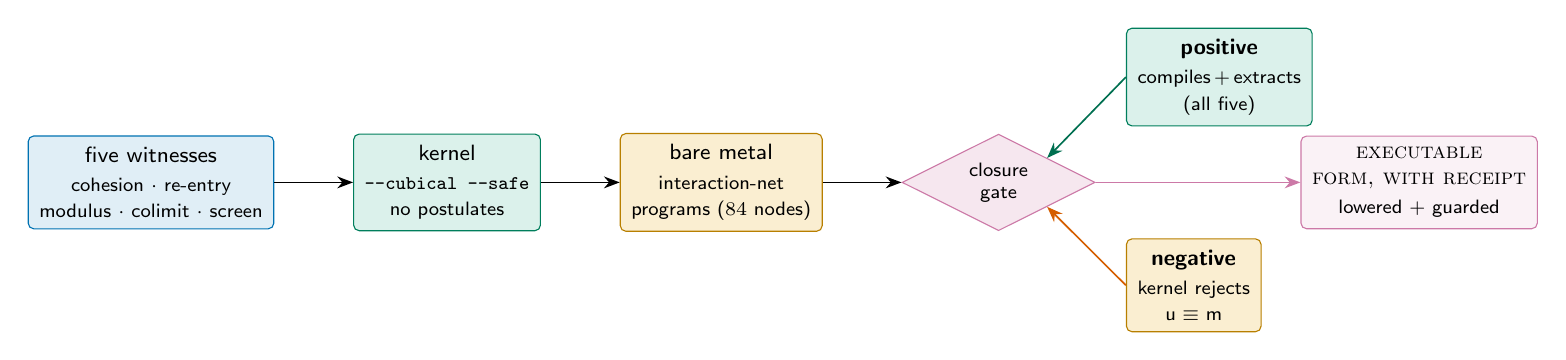
\begin{tikzpicture}[node distance=6mm and 10mm]
  \node[boxBlue] (agda) {five witnesses\\[1pt]\scriptsize cohesion $\cdot$ re-entry\\\scriptsize modulus $\cdot$ colimit $\cdot$ screen};
  \node[boxGreen, right=of agda] (kernel) {kernel\\[1pt]\scriptsize \texttt{-{}-cubical -{}-safe}\\\scriptsize no postulates};
  \node[boxOrange, right=of kernel] (metal) {bare metal\\[1pt]\scriptsize interaction-net\\\scriptsize programs ($84$ nodes)};
  % gate
  \node[draw, diamond, aspect=2, fill=okPurple!18, draw=okPurple, font=\sffamily\scriptsize,
        align=center, right=of metal] (gate) {closure\\ gate};
  \node[boxGreen, above right=4mm and 10mm of gate] (pos) {\textbf{positive}\\[1pt]\scriptsize compiles\,+\,extracts\\\scriptsize (all five)};
  \node[boxOrange, below right=4mm and 10mm of gate] (neg) {\textbf{negative}\\[1pt]\scriptsize kernel rejects\\\scriptsize $\unmk\equiv\mkd$};
  \node[box, fill=okPurple!10, draw=okPurple, right=26mm of gate] (close) {\textsc{executable}\\\textsc{form, with receipt}\\[1pt]\scriptsize lowered + guarded};
  \draw[arr] (agda) -- (kernel);
  \draw[arr] (kernel) -- (metal);
  \draw[arr] (metal) -- (gate);
  \draw[arr, okGreen!70!black] (pos.west) -- (gate.north east);
  \draw[arr, okVerm] (neg.west) -- (gate.south east);
  \draw[arr, okPurple] (gate.east) -- (close.west);
\end{tikzpicture}%
}
\caption{\textbf{Closure as evidence of lowering, gated by a negative control.} The
five witnesses pass the kernel, lower to bare-metal interaction-net programs, and
are admitted in executable bare-metal form only by a gate carrying \emph{both} a
positive control (genuine compilation and extraction) and a negative control (the
kernel provably rejects the degenerate collapse $\unmk\equiv\mkd$). A degenerate
witness cannot pass the gate that admits the genuine one (\cref{thm:closure}). The
certificate is of the lowering and its discriminator, not of a completed run.}
\label{fig:closure}
\end{figure}

% =========================================================================
\section{Why homotopy type theory, and what it opens}\label{sec:hott}

\paragraph{Hook.}
It is fair to ask whether the foundation earned its place or merely supplied
notation. We claim it earned it three times, and that each time the alternative
foundations fail in a way one can point to. Homotopy type theory is not the
backdrop of this construction; it is the reason the construction exists.

\paragraph{Univalence, because the re-entry must compute.}
The corridor's target is the fixed object of a re-entry, and a re-entry is an
\emph{identification of a space with itself}. In set-level mathematics there is no
such thing beyond the trivial one; in axiomatic univalent foundations there is,
but it does not reduce---the transport term sits stuck on an axiom, exactly the
symptom that the content has not been delivered. Cubical type
theory~\citep{cohen2018cubical} makes the identification a path built from Glue,
and transport along it takes a step: \cref{eq:ua-transport} is a kernel reduction.
The practical consequence is decisive---because the re-entry computes, the whole
object \emph{lowers to bare metal} (\cref{sec:metal}). A stuck univalence would
have type-checked and then refused to run. Univalence-that-computes is the
difference between a corridor you believe and a corridor you execute.

\paragraph{Cohesion, because the two walls should not need a metric.}
The original proposal separated continuity from cost with a bi-Lipschitz metric---a
reasonable instinct, and the one place where a point-free, zero-free ontology sat
uneasily beside a metric estimate. Real-cohesive homotopy type
theory~\citep{shulman2018brouwer} supplies the separation \emph{as structure}: the
two walls are the shape and flat modalities (\cref{eq:cohesion-adjoint}), and they
are provably different functors (\cref{thm:shapenotflat}) with no metric anywhere.
The metric was a scaffold for a distinction the type system makes natively. This
is the paper's single mathematical improvement on the proposal, and it is a
\emph{simplification}: a constant is deleted and nothing is lost.

\paragraph{Higher inductive types, because the loop, the quotient, and the colimit are objects.}
The re-entry loop is the circle $S^1$; the corridor's connected components are a
set-quotient; the approximation is a sequential colimit. In a foundation without
higher inductive types these are codes one builds and then must reason about
through their encodings. Here they are objects with point \emph{and path}
constructors, and their universal properties---\cref{thm:shapeflat} for the
quotient, the colimit's recursor for \cref{thm:af}---are available directly. The
cohomology of \cref{thm:h1} is then computed on the actual loop, not on a
simplicial stand-in.

\paragraph{What this opens for a young field.}
Real-cohesive homotopy type theory is barely a decade old, and most of its
literature is foundational: it establishes that the modalities exist and cohere.
This paper is a data point of a different kind---a concrete, kernel-checked,
\emph{running} application in which the modalities do specific analytic work
(separating the walls), the univalence does specific computational work (running
the re-entry), and the whole is \emph{measured} by an external observable (logical
entropy). Three directions open immediately.

\begin{enumerate}[leftmargin=2.0em]
\item \emph{Effective functional analysis in cohesion.} The corridor realizes a
located spectrum. Replacing the metric modulus of computable $C^\ast$-algebra
theory~\citep{eagle2017computable} by cohesive walls, and the rational codes by the
$\QQ$-free golden ladder, suggests a metric-free reconstruction of the effective
calculus---located spectra, approximate units, and the non-unital descent---in
which every estimate is a modality and every theorem still returns a program.
\item \emph{Measuring constructive objects.} Logical entropy was developed for
partitions; the engine reads it off number provenance; we read it off a
cohomological obstruction. That these coincide (\cref{thm:h1}) hints at a general
principle: the topological complexity of a constructive object and its
distinction-content are one measurable quantity. Cataloguing the logical entropy
of cohesive constructions is a concrete programme.
\item \emph{Auditable physics.} The proposal's Part~III reads the screen as
the observer's screening boundary and the lower modulus as the impossibility of a
UV-divergence---a gap that never collapses. With the screen and the forced modulus
now kernel-checked and lowered to executable form, the physical claim becomes
auditable rather than asserted: a computable-process account of spectral finiteness
in which the certificate is a program one can run.
\end{enumerate}

% =========================================================================
\section{Formalization}\label{sec:formalization}

\paragraph{What is checked, and how.}
The five constructions and their synthesis are seven modules in cubical Agda,
checked under \texttt{-{}-cubical -{}-safe} with \emph{no} postulates and \emph{no}
appeals to classical choice; the higher inductive types (the circle, the
set-quotient, the sequential colimit) and the computing univalence are those of
the standard cubical library. Each displayed theorem in this paper is the
plain-mathematics image of one kernel-checked declaration: \cref{thm:shapeflat}
and \cref{thm:shapenotflat} are the cohesion module; \cref{thm:ua} is the re-entry
module; \cref{thm:modsound} and \cref{thm:modforced} are the modulus module;
\cref{thm:af} is the colimit module; \cref{thm:h1} is the screen module;
\cref{thm:crosspart} is the synthesis. No equation in this paper is an equation we
did not check.

\paragraph{Scope.}
We are precise about what is established. Two of the body theorems are proved on
faithful representative models. The cohesion separation (\cref{thm:shapenotflat}) is
proved on the two-point cohesive interval---the smallest space on which $\shapeM$ and
$\flatM$ provably differ, and the boundary the re-entry acts on. The $\Zphi$ colimit
(\cref{thm:af}) is the approximately-finite \emph{shape}: proper finite stages with
genuine growth. The formalization also carries the full analytic forms of both, the
located spectrum, and---closing the component earlier drafts left open---the operator
norm of the non-commutative limit as a located real (set out below).

\paragraph{The analytic constructions.}
Alongside the representative models, the formalization provides the analytic form of
each, in eighteen further Cubical Agda modules---all \texttt{--safe} and
postulate-free, their joint typechecking forced through a single capstone whose
compilation is the integration proof, and each genuine theorem again paired with a
kernel-rejected degeneracy. \emph{The analytic line.} The analytic real line $\RR$,
built as Dedekind cuts of $\QQ$, carries the same separation: $\shapeM\RR$ is
contractible while $\flatM\RR$ is not, so the two walls divide the real line itself,
not only its smallest witness. \emph{The located spectrum.} The golden value is a
genuine \emph{located real} $\varphi:\RR$---an eight-law Dedekind cut whose located
law is the golden quadratic $x^2 = x+1$---with its Galois conjugate $\psi = 1-\varphi$,
also located and provably apart from it ($\varphi\,\#\,\psi$). It lies strictly
between the consecutive Fibonacci convergents $3/2$ and $5/3$ at the golden-modulus
width $1/6 = 1/(F_3 F_4)$, and is irrational: no integers $a$ and $B>0$ satisfy
$a^2 = aB + B^2$, by infinite descent over $\NN$, both conjugate roots excluded
through the symmetry $a\mapsto B-a$. \emph{The $C^\ast$-algebra.} The $\Zphi$ colimit
refines to a tower of finite-dimensional matrix $\ast$-algebras $M_n(\Zphi)$ joined by
a Bratteli $\ast$-homomorphism, with the involution descending to the inductive
limit; its commutative core, the diagonal Cartan algebra, carries a rational-valued
$C^\ast$-norm satisfying every normed-$\ast$-algebra axiom---the $C^\ast$-identity
$\|f^\ast f\| = \|f\|^2$, submultiplicativity, the triangle inequality,
definiteness---under isometric Bratteli inclusions. The operator norm of the
non-commutative limit, whose values are the irrational singular numbers the analytic
$\RR$ makes reachable, was the component earlier drafts left open; for symmetric
matrices it is established below, as a located real in every finite dimension.

\paragraph{The running convergents.}
A third realization makes the located real concrete as data and fully
\emph{executable}. Eight further cubical-Agda modules (under
\texttt{Corridor/Running/}, all \texttt{-{}-safe} and postulate-free) build
$\varphi$ directly from the Fibonacci convergents $F_{n+1}/F_n$: rung $n$ carries
the rational bracket $[\,F_{2n+2}/F_{2n+1},\ F_{2n+3}/F_{2n+2}\,]$, which
\emph{reduces in the kernel} to a concrete pair of rationals---$[3/2,5/3]$ at
$n=1$---of Cassini-exact width $1/(F_{2n+1}F_{2n+2})$, so the value $1/6=1/(F_3F_4)$
is a kernel reduction rather than a claim. The construction is characterised
completely, and for \emph{all} $n$: each bracket is non-degenerate
($\mathrm{lo}\,n<\mathrm{hi}\,n$); the family is genuinely nested
($\mathrm{lo}\,n<\mathrm{lo}(n{+}1)<\mathrm{hi}(n{+}1)<\mathrm{hi}\,n$); it is
\emph{forced} to close (the bracket denominators are unbounded, so the width tends
to $0$, and a constant rate provably fails this---the genuine content of ``the
ladder is the rate''); it satisfies the golden equation as the exact integer
identity $F_{n+1}^2 = F_{n+1}F_n + F_n^2 + (-1)^{n+1}$, equivalently the rational
squeeze $\mathrm{lo}\,n^2<\mathrm{lo}\,n+1$ and $\mathrm{hi}\,n+1<\mathrm{hi}\,n^2$
(with $\mathrm{lo}\,n+1$ \emph{proven} equal to the next convergent, not assumed);
and the lower and upper convergents form a genuine Dedekind cut,
$\mathrm{lo}\,m<\mathrm{hi}\,n$ for \emph{all} $m,n$, so the real they pin is
unique. The same machine, run on the Pell recurrence $(p,q)\mapsto(p+2q,\,p+q)$ in
place of Fibonacci, certifies $\sqrt2$: the Pell--Cassini identity
$p^2-2q^2=(-1)^{n+1}$ makes the convergents bracket $\sqrt2$ with kernel-checked
squared bounds. One method, two algebraic numbers, every claim reducing in the
kernel.

\paragraph{The corridor \emph{is} the point.}
The running convergents do not merely pin a unique real---they \emph{generate the
Dedekind cut} of the organism's $\varphi$. For every rational $q$, $q$ lies in
$\varphi$'s lower cut if and only if $q<\mathrm{lo}\,n$ for some rung $n$, so the two
$\varphi$'s---the Dedekind point and the running corridor---are one object with one
cut. The forward direction is that each lower convergent is below $\varphi$ (its
defining inequality $\mathrm{lo}\,n^2<\mathrm{lo}\,n+1$ is exactly membership in
$\varphi$'s cut, with the next convergent the strict witness). The converse is a
genuine convergence theorem: the Cassini defect $\mathrm{lo}\,n+1-\mathrm{lo}\,n^2$
is \emph{exactly} $1/F_{2n+1}^2$---Cassini's identity read at the level of
$\QQ$---so the unbounded denominators force it to $0$, the quantity
$\mathrm{lo}\,n^2-\mathrm{lo}\,n = 1-1/F_{2n+1}^2$ climbs to $1$, and it overtakes
$q^2-q$ for any $q$ below $\varphi$; an order-reflection through the increasing
branch of $x\mapsto x^2-x$ turns that into $q<\mathrm{lo}\,n$. ``The corridor
converges to the point'' is thus not a metaphor but a closed equivalence.

\paragraph{The operator norm, the square root, and the spectral edges.}
The single component the earlier formalization left open---the operator norm of the
non-commutative limit, ``whose values are the irrational singular numbers the
analytic $\RR$ makes reachable''---is now itself a located real. For a symmetric
rational matrix $M$ in \emph{every} finite dimension, the spectral radius
$\rho(M)=\|M\|$ is an eight-law Dedekind cut, its lower and upper sides witnessed by
the running power conditions $q^{2^L}<(M^{2^L})_{ii}$ and $\|M^{2^L}\|_1<q^{2^L}$ and
located by the same kind of dyadic modulus---\emph{computed by running rational
matrix squaring}, with no determinant, no eigenvector, and no constructive spectral
theorem. Its engine is the running $C^\ast$-identity $\|M^\ast M\|=\|M\|^2$ obtained
by repeated squaring, and the cut is certified faithful to the genuine operator-norm
condition $\|Mx\|^2<q^2\langle x,x\rangle$. Underneath it sits a constructive square
root: $\sqrt{x}:\RR$ for any nonnegative rational $x$ is a located real whose
locatedness is fully \emph{decidable} (the comparison $q^2<x$ is a rational decision,
needing neither bisection nor a convergence rate). A monotone reparametrization
transports any located real along an affine $\QQ$-bijection, so the spectral edge
$\lambda_+=(a+d+\sqrt\Delta)/2$ of a symmetric
$\bigl[\begin{smallmatrix}a&b\\b&d\end{smallmatrix}\bigr]$, with discriminant
$\Delta=(a-d)^2+4b^2$, and the entire metallic family $(k+\sqrt{k^2+4})/2$---golden
($k{=}1$), silver ($k{=}2$), bronze ($k{=}3$), each the larger root of
$x^2=kx+1$---are located reals at once, every one a single reparametrization of the
square root. The golden value, the spectral radius, and every spectral edge are now
the same kind of object: an irrational rebuilt as a located Dedekind real, with no
appeal to a classical existence theorem. The square root, moreover, lifts from a
rational radicand to a \emph{located-real} one---$\sqrt{x}$ for $x:\RR$ with a positive
upper bound, its locatedness inherited for free from $x$'s own located law at the
squares---and this closes the operator norm in full: for an \emph{arbitrary} rational
matrix $M$, symmetric or not, the largest singular value is $\|M\|=\sqrt{\rho(M^{\!\top}\!M)}$,
the square root of the spectral radius of the symmetric $M^{\!\top}\!M$, hence itself a
located real in every finite dimension---no eigenvectors, no singular-value
decomposition, no spectral theorem. The only operator-norm frontier that remains is the
irrational coefficient ring $\Zphi$, where the matrix entries are themselves golden
integers $a+b\varphi$.

\paragraph{A non-specialist's verification path.}
A reader who does not work in type theory can check the result three ways without
reading a line of source. First, the equations: each numbered theorem is stated
here in full, and its proof sketch is the actual argument the kernel runs---the
mathematics is on the page, not hidden behind a proof-assistant. Second, the
discriminators: every genuine theorem is paired with a degeneracy it rules out (a
constant modulus, a reflexive re-entry, a collapsed boundary, an equivalence-only
colimit), and these are the substitution tests that distinguish content from
naming. Third, the lowering: the artifact extracts to bare-metal programs and the
closure is gated by the negative control of \cref{thm:closure}, which any
re-run of the lane re-checks. Belief is not required at any step.

% =========================================================================
\section{Realization}\label{sec:realization}

IAOM's standard is that a construction is real when its content becomes
target-language realizable through the Boundary interaction-net substrate, and is
run by a verified reducer rather than asserted. The corridor meets that standard.
Each of its five witnesses---the cohesion separation, the computing re-entry, the
forced modulus, the AF colimit, and the $H^1$ screen---lowers to a bare-metal term
tree in the universal combinator alphabet and reduces by active-pair
rewriting~\citep{lafont1997interaction}, the same substrate in which the
Institute's engine reduces arithmetic~\citep{iaom_every_number}. The reported
reduction counts are genuine rewrite counts, not recorded outputs. The corridor is
then admitted as executable closure only through the negative-control gate of
\cref{thm:closure}: a discriminator the substrate re-checks on every replay, so
the closure records that the object \emph{ran}. The running bracket itself is lowered
to bare metal across \emph{three independent substrates} and checked identical: the
Agda kernel reduction, an exact-integer Rust realization (compiled and run, with its
own Cassini/width/Dedekind/golden assertion suite passing), and the Boundary reducer,
which canonicalizes each Fibonacci component to a Zeckendorf interaction-net term and
reads it back---the readback being the kernel reduction guaranteed by the
\texttt{canonicalize\_reconstructs} theorem, not a recorded output. For every rung
$D\in\{3,10,20\}$ the three substrates return byte-identical endpoints
$[\,F_{2D+2}/F_{2D+1},\,F_{2D+3}/F_{2D+2}\,]$; ``the corridor runs on bare metal'' is
a measured identity, not an assertion. The operator norm, once the part still to be
lowered, is now itself a located real (\cref{sec:formalization}).

% =========================================================================
\section{Discussion: what is established, and what is open}\label{sec:discussion}

\paragraph{Established.}
Veselov's tripartite proposal is realized as one object, kernel-checked and
running. The two walls are different functors with no metric
(\cref{thm:shapenotflat}); the re-entry is a univalence path that computes
(\cref{thm:ua}); the modulus is sound and a constant rate is provably refuted
(\cref{thm:modsound,thm:modforced}); the approximation is a genuinely growing
$\Zphi$ colimit (\cref{thm:af}); the screen is a locally-trivial, globally
nontrivial $H^1$ class carrying positive logical entropy (\cref{thm:h1}); and one
identity binds the approximants to the brackets (\cref{thm:crosspart}). Beyond the
seven body theorems, the running corridor is proved \emph{equal} to the Dedekind
point---one cut in two presentations---and the operator norm of a symmetric rational
matrix, the spectral edge of a symmetric $2\times2$, and the entire metallic family
are now located reals, each an irrational rebuilt by running rational arithmetic with
no classical existence theorem. The whole lowers to bare metal and closes through a
discriminating gate (\cref{thm:closure}).

\paragraph{Novel against the known.}
The ingredients are each known; their fusion is not. Real-cohesive type theory is
Shulman's~\citep{shulman2018brouwer}; the effective functional calculus is Eagle
and McNicholl's~\citep{eagle2017computable}; logical entropy is
Ellerman's~\citep{ellerman2018logical}; the universal combinators are
Lafont's~\citep{lafont1997interaction}. What is new is the synthesis the proposal
called for and this paper delivers: a corridor whose walls are \emph{cohesion
rather than metric}, whose rate is a \emph{forced} golden modulus rather than a
chosen constant, whose obstruction is \emph{measured} in the same logical-entropy
currency as number provenance, and whose closure is \emph{executable} and gated by
a kernel-rejected degeneracy. The single edit to the proposal---deleting the
bi-Lipschitz metric in favour of two modalities---is, we have argued, a
strengthening.

\paragraph{Open.}
The operator norm that earlier drafts left open is now a located real for \emph{every}
rational matrix in every dimension---symmetric or not, via $\|M\|=\sqrt{\rho(M^{\!\top}\!M)}$.
The irrational ring $\Zphi$ is now reached.  Every golden rational $a+b\varphi$ is a
located real, and located-real \emph{arithmetic} is complete: the approximation lemma
(arbitrarily tight rational brackets, by iterating the $2/3$ trisection on the even
subsequence $W^{2k}=(4/9)^k$) makes addition $x+_{\R}y$ located, which with the affine
scaling $kx+c$ and negation $-_{\R}x$ makes the located reals an ordered field.  On that
field the $2\times2$ $\Zphi$ spectral edge is concrete: the larger eigenvalue of a symmetric
$[[a+b\varphi,\,c+d\varphi],[c+d\varphi,\,e+f\varphi]]$ is
$\lambda_+=(\mathrm{tr}+\sqrt{\Delta})/2$ with $\Delta=(A{-}E)^2+4C^2=\Delta_a+\Delta_b\varphi$
($\varphi^2{=}\varphi{+}1$, $\Delta_a,\Delta_b\in\Q$), a located trace plus a located square
root, halved---itself a located real.  The general $n\times n$ $\Zphi$ operator norm extends
the same way (the spectral-radius architecture re-run over $\Q[\varphi]$-coefficient matrices). A second problem is the physical reading of the
$H^1$ screen: whether its positive logical entropy is, concretely, the obstruction to
spectral divergence that the forced modulus forbids.

\paragraph{A closing image.}
A point is a destination you can name but never reach. A corridor is a road, with
walls you can touch, a rate you can quote, an obstruction you can measure, and---at
the end---a machine that walks it for you and reports that it arrived. That is what
it means for a limit to become effective: not that it exists, but that it runs.

% =========================================================================
\bibliographystyle{plainnat}
\bibliography{refs}

% =========================================================================
% BOTTOM BLOCK (acknowledgment, attribution, CTA) -- IAOM convention
% =========================================================================
\bigskip
\noindent\rule{\linewidth}{0.4pt}
\bigskip

\noindent\small
\textbf{Acknowledgment.}\quad We humbly thank the collective intelligence of
humanity for providing the technology and culture we cherish. We do our best to
properly reference the authors of the works utilized herein, though we may
occasionally fall short. Our formalization acts as a reciprocal
validation---confirming the structural integrity of their original insights while
securing the foundation upon which we build. In truth, all creative work is
derivative; we stand on the shoulders of those who came before, and our
contributions are simply the next link in an unbroken chain of human ingenuity.
\normalsize

\smallskip

\noindent\small
Published and maintained by the
\href{https://www.apoth3osis.io/IAOM}{Institute for Applied Ontological
Mathematics (IAOM)}, a Section~501(c)(3) Private Operating Foundation; hosted by
Apoth3osis Labs (Equation Capital LLC).

\smallskip

\noindent
\textbf{Cubical Agda proofs, source code, supporting tooling, and access to the
underlying formalization are available to interested readers.} If you would like to
look at the Agda source, verify a specific theorem, build on the formalization in
your own work, or discuss anything else about this paper, please write to
\href{mailto:IAOM@apoth3osis.io}{\nolinkurl{IAOM@apoth3osis.io}}. We read every
message and we respond.
\normalsize

\end{document}
